\subsection{Impulse Response Coefficient Based on Linear Model}
The discrete time state space model is now used to determine the impulse response. The response is determined as seen in \cref{eq:Markov} in \cref{sec:Imp_res}. The parameters can be seen in the below figure where they are compared to the response determined on basis of the transfer function.
\begin{figure}[H]
    \centering
    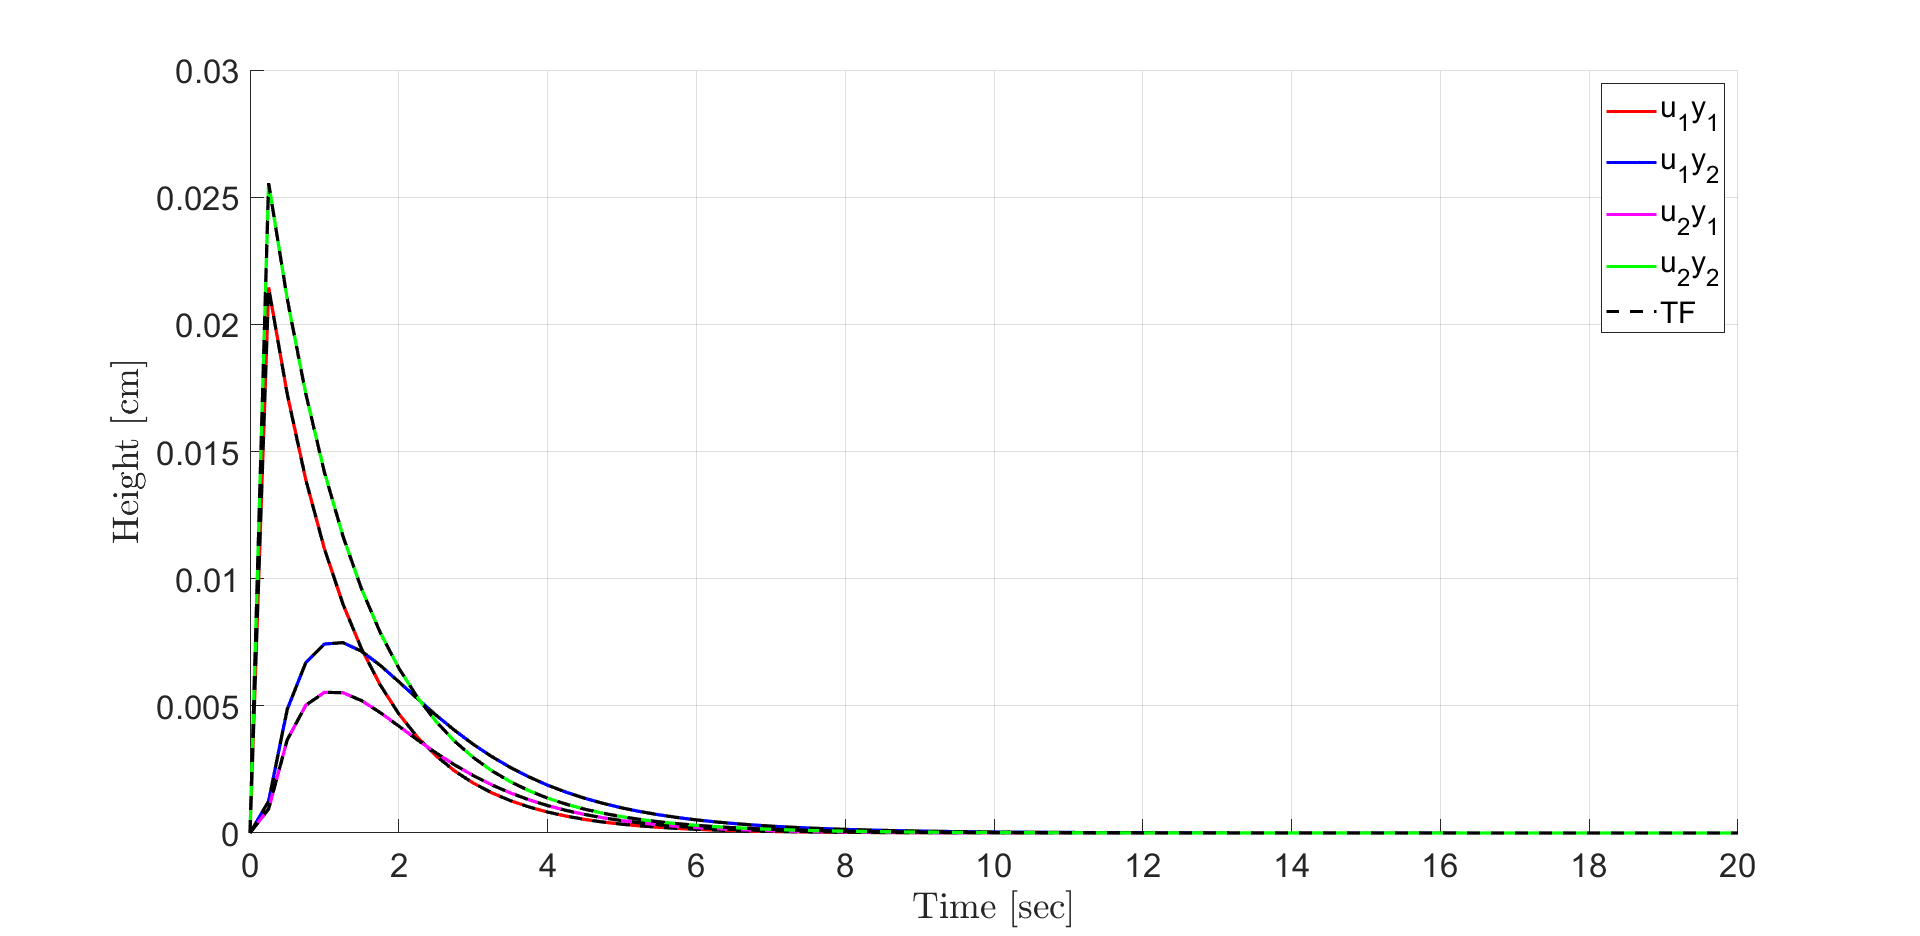
\includegraphics[width=1\textwidth]{Figures/Pr4.6_Markov_compare.png}
    \caption{Impulse reponse - Comparison}
    \label{fig:Markov_compare}
\end{figure}
The black-dotted line indicates the previous determine response based om the transfer functions. It can be seen that the difference between the response based on the discretized model and the transfer functions is more or less zero. It is expected that if the response was compared for larger step responses, a larger deviation would be expected as consequence of the linearization.